
\documentclass[11pt,fleqn]{article} 
\usepackage[margin=0.8in, head=0.8in]{geometry} 
\usepackage{amsmath, amssymb, amsthm}
\usepackage{fancyhdr, wrapfig} 
\usepackage{palatino, url, multicol}
\usepackage{graphicx, pgfplots} 
\usepackage[all]{xy}
\usepackage{polynom} 
%\usepackage{pdfsync} %% I don't know why this messes up tabular column widths
\usepackage{enumerate}
\usepackage{framed}
\usepackage{setspace}
\usepackage{array,tikz}

\pgfplotsset{compat=1.6}

\pgfplotsset{soldot/.style={color=black,only marks,mark=*}} \pgfplotsset{holdot/.style={color=black,fill=white,only marks,mark=*}}


\pagestyle{fancy} 
\lfoot{}
\rfoot{\S 3.6}

\begin{document}
\renewcommand{\headrulewidth}{0pt}
\newcommand{\blank}[1]{\rule{#1}{0.75pt}}
\newcommand{\bc}{\begin{center}}
\newcommand{\ec}{\end{center}}
\renewcommand{\d}{\displaystyle}

\vspace*{-0.7in}

%%%%%%%%%intro page
\begin{center}
  \large
  \sc{Section 3.6: Numerical Integration}\\
\end{center}

\bigskip
\begin{minipage}{0.55\textwidth}
We will try to estimate the definite integral
    $$\int_0^2 \cos(x^2) \,dx$$
I do not know how to do it by hand exactly.  (\emph{Feel free to try?})  However, we can graph the function $y=\cos(x^2)$.  Eyeballing the graph at right, the area above the axis is about 1 and the area below is about 1/2, so we expect a final integral of about 1/2.
\end{minipage}

\vspace{-45mm}
\hfill 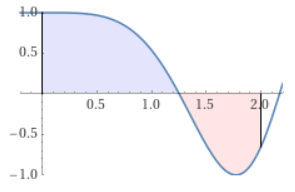
\includegraphics[width=0.35\textwidth]{figs/cosxx.png}

\medskip
\begin{enumerate}
\item Write down the Midpoint Rule $M_4$ for this integral, with $n=4$ subintervals.  (\emph{What are the values of $\Delta x$ and the points $m_i$?})

\vspace{1in}

\item Use a calculator to evaluate $M_4$.  Round your estimate to 4 decimal places.

\vfill

\item Write down the Trapezoid Rule $T_4$ for this integral, with $n=4$ subintervals.  (\emph{What are the values of $\Delta x$ and the points $x_i$?})\\

\vspace{1in}

\item Use a calculator to evaluate $T_4$.  Round your estimate to 4 decimal places.

\vfill
\newpage
\item Write down Simpson's Rule $S_4$ for this integral, with $n=4$ subintervals.  (\emph{What are the values of $\Delta x$ and the points $x_i$?})

\vspace{2in}

\item Use a calculator to evaluate $S_4$.  Round your estimate to 4 decimal places.

\vfill

\item In Matlab, the command
\begin{verbatim}
    >> integral(@(x) cos(x.^2),0,2)
\end{verbatim}
gives the 0.461461462433216 as an estimate.  Using this number as the exact value of the integral, determine the \emph{absolute} error for each of the three estimates $M_4$, $T_4$, $S_4$.
\vfill
\end{enumerate}
\end{document}
